%% manuscript produces a one-column, double-spaced document:
\documentclass[12pt, manuscript]{aastex}
\usepackage{graphicx}
\usepackage{hyperref}
%\usepackage[most]{tcolorbox}
%\usepackage{setspace}
%\usepackage{footmisc}
%\renewcommand{\footnotesize}{\small}

\begin{document}


\title{AKARI and Spinning Dust Emission\\
A look at microwave dust emission via the Infrared}

\author{Aaron Christopher Bell}
%\affil{University of Tokyo,
%Bunkyo, Tokyo, Japan, 113-0033;}
%\email{abell@astron.s.u-tokyo.ac.jp}

%\keywords{AME, spinning dust, PAH bands, AKARI}

\maketitle

\chapter*{Abstract}
\addcontentsline{toc}{chapter}{Abstract}
The anomalous microwave emission (AME) still lacks a conclusive explanation.  This excess of emission, roughly between 10 and 50~GHz, tends to defy attempts to explain it as synchrotron or free-free emission. The overlap with frequencies important for cosmic microwae background explorations, combined with a strong correlation with interstellar dust, drive cross-disciplinary collaboration between interstellar medium and obervational cosmology. The apparent relationship with dust has prompted a ``spinning dust'' hypothesis:  electric dipole emission by rapidly rotating, small dust grains. Magnetic dipole emission by grains with magnetic inclusions (``magnetic dust''), while less suppported, has not been ruled out. Even assuming a spinning dust scenario, we are far from concluding which category of dust contributes. The typical peak frequency range of the AME profile implicates grains on the order of ~1nm. This points to polycyclic aromatic hydrocarbon molecules (PAHs). We use data from the AKARI/Infrared Camera (IRC; \citet{irc07}), due to its thorough PAH-band coverage, to compare AME from the \cite{planck15X}. astrophysical component separation product) with infrared dust emission. We look also at infrared dust emission from other mid IR and far-IR bands. The results and discussion contained here apply to an angular scale of approximately 1$^{\circ}$. In general, our results support an AME-from-dust hypothesis. We look both at $\lambda$~Orionis, a region highlighted for strong AME, and find that certainly dust mass correlates with AME, and that PAH-related emission in the AKARI/IRC 9~$\mu$m band may correlate slightly more strongly. These results are compared to an all-sky analysis, where we find that potential microwave emission component separation imperfections among other issues, make an all-sky, delocalized comparsion very challenging. In any case the AME-to-dust correlation persists even in the all-sky case, but tests of relative variations from different dust SED components are largely inconclusive. We emphasize that future efforts to understand AME should focus on individual regions, and a detailed comparsion of the PAH features with the variation of the AME SED. Further all-sky analyses seem unlikely to help resolve this issue. Non-PAH carriers of the AME, such as nanosilicates, cannot be ruled out either.

All-sky astronomy is not new. Indeed, the notion of capturing a particular "object" or "source" with a camera and saving it for later investigation would be completely alien to the first astronomers and astronavigators. Absence of telescopes forced us to describe the sky in terms of its larger patterns, brightest characters. What is new however, is the notion of preparing an archive of the sky itself for not only the research whims of a single investigator, team, institute, or even a single nation- rather, all-sky surveys tend to be international endeavors in their production, and even more so in their utilization.

This is especially true in the context of infrared astronomy, a field which was essentially non-existant as recently as the 1950s \citep{johnson66} \footnote{1920s, if we judge by the first IR observations}. Compare this to visible wavelength- a field so old we name it after the bio-evolutionary advent of sight, itself. Even radio astronomy with its own logistical and technological challenges, has been around since at least 1932.

`` Johnson+ 1966 p.194: "It is now plain that about 75\% of the data we would like to have can be obtained from good ground-based sites"
% ...p.1 "The Far Infrared, from 4 to 22 um''

Despite the above claim from \citep{johnson66}, astronomers were apprently not content to be constrained by atmospheric IR windows, even from the best of ground-based sites. Or perhaps interests have shifted so dramtically since 1966, that all of the investigations enabled by rocket-based, space-based, even Boeing 747-based IR astronomy would have bored 75\% of astronomers in the '60s.

\chapter{Data Sources}
  \label{ch:datasources}

  \section{A collection of skies}
    This work relies completely on all-sky surveys. All of the maps utilized are photometric-band infrared maps, except for the AME data, which is an all-sky component separation analysis product, from the Planck Collaboration's efforts to separate galactic foregrounds from the CMB.


    \begin{table}[h]
      \label{tab:data}
      \caption{Observational data sources used in this article}
      \centering
        \begin{tabular}{lrrrrr}
        \hline\hline
        Instrument & Central Wavelength & FWHM & Cali & Reference \\
        \hline
        AKARI/IRC & 9~$\mu$m  &  \~{}10$"$ & \textless 10\%   & \tablefootnote{\citep{ishihara10}} \\
        AKARI/IRC & 18~$\mu$m & \~{}10$"$  & \textless 10\%     & '' \\
        AKARI/FIS & 65~$\mu$m  & 63$"$ & \textless 10\% & \tablefootnote{\cite{doi15,takita16}} \\
        AKARI/FIS & 90~$\mu$m  & 78$"$ & \textless 10\%   & '' \\
        AKARI/FIS & 140~$\mu$m & 88$"$ & \textless 10\%   & '' \\
        AKARI/FIS & 160~$\mu$m & 88$"$ & \textless 10\%   & '' \\
        IRAS/IRIS & 12~$\mu$m   & 4.0$'$ &   \textless 5.1\%       & \tablefootnote{\cite{iris05}} \\
        IRAS/IRIS & 25~$\mu$m   & 4.0$'$ &    \textless 15.1\%      & ''\\
        IRAS/IRIS & 60~$\mu$m   & 4.2$'$ &    \textless 10.4\%      & '' \\
        IRAS/IRIS & 100~$\mu$m  & 4.5$'$ &   \textless 13.5\%       & '' \\
        Planck/HFI & 345~$\mu$m & 4.7$'$ & & \tablefootnote{\cite{hfi14viii}} \\
        Planck/HFI & 550~$\mu$m & 4.3$'$& & '' \\
        \hline
      \end{tabular}
    \end{table}

  \subsection{Primary band of interest}\footnote{Not to be confused with ``The band primarily interested'' in dust, Queen.}
    The AKARI/IRC 9~$\mu$m band (A9) provides uniquely complete coverage of the PAH bands at 6.2, 7.7, 8.6, and 11.2~$\mu$m, and may be an excellent tool for testing PAH-related hyoptheses on an all-sky basis. The combination of A9 with W12 and/or I12 may be especially insightful. In total, we employ all-sky maps from 12 photometric bands, spanning the wavelength range of 6.9~$\mu$m to 550~$\mu$m\footnote{Planck bands are named according to their central frequency, not wavelength.}

  \section{Infrared Data}
    \subsection{AKARI}
       The AKARI infrared space telescope revealed an entire sky of infrared light, from the mid to far infrared, via two instruments \citep{akari07} the Infrared Camera (IRC)\citep{irc07} and the Far Infrared Surveyor (FIS) \citep{fis07}.

       \paragraph{AKARI/IRC PAH feature coverage}
         The IRC's 9~$\mu$m band all-sky map demonstrates the abundance of the PAH bands carrier in the Milky Way \citep{ishihara10}. Figure \ref{fig:relSpectralResponse_MIR} shows the coverage of the MIR bands along with an example galactic cirrus SED. The 9~$\mu$m band uniquely covers major ionized PAH features at 6.2 and 7.7~$\mu$m; as well as neutral PAH features at 8.6 and 11.2~$\mu$m across the entire sky \citep{irc07}. The IRAS 12~$\mu$m band covers the 11.2 and 8.6~$\mu$m features, and the similarly-shaped WISE~12~$\mu$m band covers primarily the 11.2~$\mu$m feature.

         \paragraph{In-band conribution from PAHs}
           According to this distribution of PAH features across the response filters, it is expected that the IRC 9~$\mu{}$m band is most dominated by PAH emission even with increasing $G_0$. These contributions remain relatively constant out to a $G_{0}$ of about 100, with the contribution from warm dust becomming a larger factor for the IRAS 12~$\mu$m and WISE 12~$\mu$m bands. Thus, according the the DL01 template, IRC 9~$\mu$m should have the highest contribution from PAHs out to extreme radiation fields.

          \paragraph{Potential to trace PAH ionization}
            Fig. \ref{fig:inband_ionfrac_ratios} demonstrates how the band ratios of the IRC 9um band vs. the other MIR bands change with different modeled PAH ionization fractions (determined using the DustEM default model template, by \cite{dustem11}. This band ratio can be determined, because the IRC9 filter is more sensitive to ionized PAH features, relative to IRAS12 or to WISE12.
           IRC 9~$\mu$m shows a larger contribution from ionized PAHs, by about 16 percent, and a conversely smaller contribution from neutral PAHs.

       \begin{figure*}
       \label{fig:relSpectralResponse_MIR}
       \centering
       \includegraphics[width=150mm]{../Plots/RelSpectralResponse_MIR.png}
       \caption{Relative spectral response curves of the MIR bands used in this study, AKARI/IRC 9~$\mu$m, IRAS 12~$\mu$m, WISE 12~$\mu$m, AKARI 18~$\mu$m, and  IRAS 25~$\mu$m. AKARI/IRC 9~$\mu$m, IRAS 12~$\mu$m, WISE 12~$\mu$m bands are dominated by PAH emission.}
       \end{figure*}


       \begin{figure*}
       \label{fig:inband_ionfrac_ratios}
       \centering
       \includegraphics[width=150mm]{../Plots/band-ratio-multiple.pdf}
       \caption{Ionization fraction of PAHs vs. band ratios of IRAS12 and 25, and WISE 12 and 25~$\mu$m bads vs. the AKARI 9~$\mu$m band, for three ISRF strengths: Top: $G_{0} = 100$, Middle: $G_{0} = 1000$, and Bottom: $G_{0} = 10000$. These ratios are determined by assuming the SED template if \cite{dustem11} }
       \end{figure*}

        We utilize the most recent version of the IRC data (Ishihara, et al., in prep.) This version has had an updated model of the Zodiacal light, fitted and subtracted. The details of the improved Zodi-model, which offers an improvement over that used for the IRAS all-sky maps, are given in \cite{kondo16}.



      The AKARI Far Infrared Surveyor (FIS) gives us photometric data around the peak of the typical thermal dust SED. FIS was equipped with four wavebands: two narrow bands centered at 65~$\mu$m and at 160~$\mu$m, and two wide bands at 90~$\mu$m and at 140~$\mu$m. An all-sky survey was carried out at each band \citep{kawada07}, and the processed maps have been publicly released \citep{doi15}.

       The Planck Space Observatory (Planck) High Frequency Instrument (HFI) all-sky maps, spanning 100 to 857~GHz \citep{hfi14viii} help constrain the far IR dust emissivity. This study utilizes the 857~GHz (345~$\mu$m) and 545~GHz (550~$\mu$m) bands.

       Data from the Infrared Astronomical Satellite \citep{iras84} all-sky surveys are used to supplement the similarly-centered AKARI photometric bands. The IRAS 12~$\mu$m band is similar to the AKARI 9~$\mu$m band in terms of the sky coverage, central wavelength, and especially in that both surveys are heavily dominated by zodiacal light. We use the Improved Reprocessing of the IRAS Surveys (IRIS) \citep{iris05}, which use undergone a zodiacal-light removal. The Zodiacal light model, however differs between the two bands. The IRAS Zodi-subtraction is primarily based on the \cite{kelsall98} model.

  \section{Planck COMMANDERAME Parameter Maps}

       We utilize the COMMANDER-Ruler astrophysical component separation maps, from the Planck Collaboration's Public Data Release 2 (hereafter, PR2). These contain estimates of known microwave foreground components (free-free, synchrotron, thermal dust emission contributions to the Planck photometric bands. Details of the foreground contribution estimates are given in \cite{planckXII}. We will first describe the 'non-AME' components, so as to not give any indiciation that their estimation is trival.

       \begin{figure*}
         \label{fig:PCCS_corrmatrix}
         \includegraphics[width=\textwidth]{../Plots/ch_datasources/PCCS_corrmatrix.pdf}
         \centering
         \caption{All-sky map of the peak frequencies of the varying component $AME_{var}$, corresponding to Fig. \ref{fig:AME_commander_freqdist}.}
       \end{figure*}

       \subsection{Synchrotron}
        While the Planck observations themselves do limit our resolution when assessing the AME - it is in fact the primary constraint on synchrotron emission, 408~MHz map by \cite{haslam82} that is the major resolution limiting factor. While an impressive, pioneering effort for to reveal the low-frequency sky, \citep{haslam82} is limited to an appriximately 1 degree resolution. The map also contains
        many artifacts. For the time being however, it is still the most synchrotron-dominated all-sky map available, and for this reason PC15X included it in their COMMANDER component separation. The final synchrotron product produced by COMMANDER (hereafter, PCSync) highly resembles the \citep{haslam82} map, however it is also demonstrated PCSync does not fully capture the synchrotron signal. This can be visualized by inspecting the PCAME:PCdust ratio map (see Fig. \ref{fig:R_PCAMEtoPCdust}), which \cite{hensley17} describe as containing synchrotron emission patterns at high latitudes.

        \begin{figure*}
        \label{fig:R_PCAMEtoPCdust}
        \centering
        \includegraphics[width=\textwidth]{../Plots/ch_datasources/R_PCAMEtoPCRad.pdf}
        \caption{All-sky map of the ratio of two COMMANDER components- the frequency-varying AME component divided by the intensity of thermal dust emission at 545~GHz. }
        \end{figure*}

       \subsubsection{Free-free emission}
        Unlike the PCSync component, the fitting of the Planck COMMANDER free-free component map (hereafter, PCff) does not employ any free-free dominated emisison map.\footnote{The Planck AME paper, \cite{planckXV}, had employed the H-$\alpha$ map by \cite{wham98}}.

      \subsection{Thermal dust emission}

      ``Thermal dust emission'' in the COMMANDER context refers to dust emission in the Rayleigh Jeans-regime, as the COMMANDER fitting does not include photometric constraints on the thermal emission peak, or consider small grain emission on the Wiens side.

       \subsection{COMMANDER-AME: Peak Frequency Distribution}

        $I_{AME}\nu_{var}$
        In addition, there is an ``AME component map'', which presumes that AME originates from spinning dust. While acknowledging that such a decomposition lacks a physical justfication, \cite{planck15X} break the AME into two components: a spatially varying peak frequency component, and a spatially constant peak frequency component. However as seen in Fig. \ref{fig:AME_commander_freqdist}, virtually all of the fitted peak frequncies for $AME_{var}$ beyond the reach of WMAP and Planck. Only the fitted global frequency, 33.5~GHz for the spatially constant component, is covered.


        \begin{figure*}
          \label{fig:AME_commander_freqdist}
          \includegraphics[width=\textwidth]{../Plots/ch_intro/AME_commander_freqdist.pdf}
          \centering
          \caption{The peak frequencies of the varying component $AME_{var}$.  The pink shaded region indicates frequencies not covered by either WMAP or Planck The green line at 33.5~GHz indicates the peak frequency of $AME_{fix}$.}
        \end{figure*}

        \begin{figure*}
          \label{fig:PCAME_var_freq.pdf}
          \includegraphics[width=\textwidth]{../Plots/ch_datasources/PCAME_var_freq.pdf}
          \centering
          \caption{All-sky map of the peak frequencies of the varying component $AME_{var}$, corresponding to Fig. \ref{fig:AME_commander_freqdist}.}
        \end{figure*}

        %The next figure shows the all-sky ratio map, of $AME_{var}:AME_{fix}$. That is, the ratio of the integrated intensities of these components, rather than the intensities given directly in the COMMANDER maps.
        The COMMANDER maps give each component's intensity at a different ``reference frequency'' (corresponding to photometric bands). In other words, the COMMANDER AME intensities are not peak intensities. Moreover they are intensities calculated for a single template spinning dust spectrum- but one that has been log-log translated to fit the observations (a demonstration of such shifted templates, for a common ``reference intensity'' at a common ``reference frequency'', is shown in Fig. \ref{fig:AME_commander_freqshift_templ}). The physical paraneters in the spinning dust model, ``spdust'' are not varied.

        \begin{figure*}
          \label{fig:AME_commander_freqshift_templ}
          \includegraphics[width=\textwidth]{../Plots/ch_datasources/AME_commander_freqshift_templ.pdf}
          \centering
          \caption{Spdust template spinning dust profiles fitted by PC15 when calculating $AME_{var}$.  The reference frequency, 22.8~GHz is indicated by the vertical green line. Each template has the same $AME_{var}$ amplitude of 100~$\mu$K, indicated by the horizontal green line, plotted to highlight the potential deviation between $AME_{var}$ and the actual peak intensity. }
        \end{figure*}

        For these reasons, we are very cautious in deriving conclusions from comparisons with the COMMANDE AME map. Indeed, the authors themselves include a similar disclaimer. However since there is currently no better all-sky component separation available\footnote{Indeed, improving on the COMMANDER AME map would be extremely difficult without lower frequency constraints and/or higher resolution observations of not only the AME itself but the contribution from synchrotron and free-free emisson.}, and carrying out a spinning dust modeling and component separation is beyond the scope of this work, we proceed with care.


  \section{All-sky Data Processing}

        The HFI, FIS, and IRIS maps used here are downloaded from their respective online repositories, as all-sky HEALPix\footnote{HEALPix core software is described at \url{http://healpix.sourceforge.net}. The HEALPIx python package ``healpy'' used in this work is available at: \url{https://github.com/healpy/healpy}} maps \citep{gorski05}.   NSIDE 2048 maps. In the case of the IRC maps, we first create HEALPix maps from the 4,857 all-sky survey tiles using the Aladin all-sky data visualization platform \citep{bonnarel00}. NSIDE 2048 implies an average pixel spacing of 1.7$'$. The maps are then degraded to NSIDE 1024 before carrying out a Gaussian-beam smoothing to a 1$^{\circ}$ FWHM \footnote{To be clear, maps are converted first to spherical harmonic space, smoothed, and transformed back to position space using - steps carried about by the smoothing function contained in the healpy python package}. Following the smoothing process, the maps are degraded once more to NSIDE 256, or 15arcmin pixel-width \footnote{HEALPix pixel scale rebinning carried out with healpy.ud\_grade}. The value of each of the larger NSIDE 256 pixels, comes from the mean of its parent NSIDE 1024 pixels. The purpose of this processing is to ensure that all of the maps have the same resolution as the PR2 AME map.

\chapter{All-sky Analysis}
\label{sec:analysis}

    We inspect the IR abd AME data in 3 approaches, relying on HEALPix maps at ~1$^{\circ}$ angular resolution. We start with an all-sky AME to IR comparison, looking for global patterns among all pixels (except those within 10$^{\circ}$ of the ecliptic plane.) 2) Next we show a more regionalized comparison, looking at the set of AME-prominent galactic clouds identified by the \cite{planckXV}. As much as possible, we maintain comparability between their IRAS-Planck based result, and our result which adds-in AKARI data and dust SED fitting. 3) Lastly, we highlight the $\lambda$~Orionis molecular ring \citep{maddalena86,maddalena87}, a particular AME-dominated region with resolvable structure even at ~1$^{\circ}$ angular resolution.

\section{All-sky Pixel Domain Analysis}

	In order to look more closely at the variations between the individual bands' maps, we include a pixel-by-pixel analysis. Figure \ref{fig:AMEvsDust_allsky_allbands} shows the result of such a comparison, for each of the 18 bands sampled. The AME data comes from the PR2 AME map.

    To keep our analysis comparable to previous works, we exclude pixels within 10$^{\circ}$ of the ecliptic plane, where the Zodi-residuals can be a problematic (especially in the MIR.)

     Figure \ref{fig:AME_IR_crosscorr_allbandsg} visualizes the cross-correlation matrix for each of the IR bands. The AME does not show a strong correlation with other bands at $|l|>10$. At $|l|<10$, the FIR bands show stronger correlation. The PAH-tracing bands show a stronger correlation than bands at 18 to 60~$\mu$m, but weaker than AME vs. the FIR bands.

  To understand how these trends may vary across the sky, we repeat the correlation analysis along 1$^{\circ}$ width latitude strips. For each degree of $b$, we cross correlate the Planck modified blackbody fitting results vs. the AME and the AKARI 9~$\mu$m intensity. (This comes with the geometrical caveat that the higher latitude bins have fewer samples.) The results of this comparison are shown in \ref{fig:PlanckModBBvsAMEandA9_bins}. Fig. \ref{fig:PlanckModBBvsAMEandA9_bins}) shows the result with longitude strips. The $l$ based comparison produces a consistent ranking of the correlation strengths all longitudes. There is an unexplained variation between $b = 200$ and 250.

  Finally, we produce an all-sky correlation map. From the NSIDE 256 input maps of each of dust temperature $T$, radiance $R$, and emissivity index beta, and $I 9~\mu$m, we produce NSIDE 16 maps of $S$ for correlation strength vs. AME. These maps are shown in Fig. \ref{fig:Spearman_Map_nside16_AMEtoMBBandA9}.

      \begin{figure*}
        \label{fig:AME_IR_crosscorr_allbandsg}
        \includegraphics[width=185mm]{../Plots/all_bands_corr_matrix_wAME_spearman.pdf}
        \centering
        \caption{ALL-SKY cross-correlation matrix for the 18 infrared bands sampled, and the AME map. THe color-scale indicates the Spearman rank ($S$). Results are based on the full sky (excluding pixels within 10$^{\circ}$ of the ecliptic plane).}
      \end{figure*}

      \begin{figure*}
        \label{fig:AMEvsDust_allsky_allbands}
        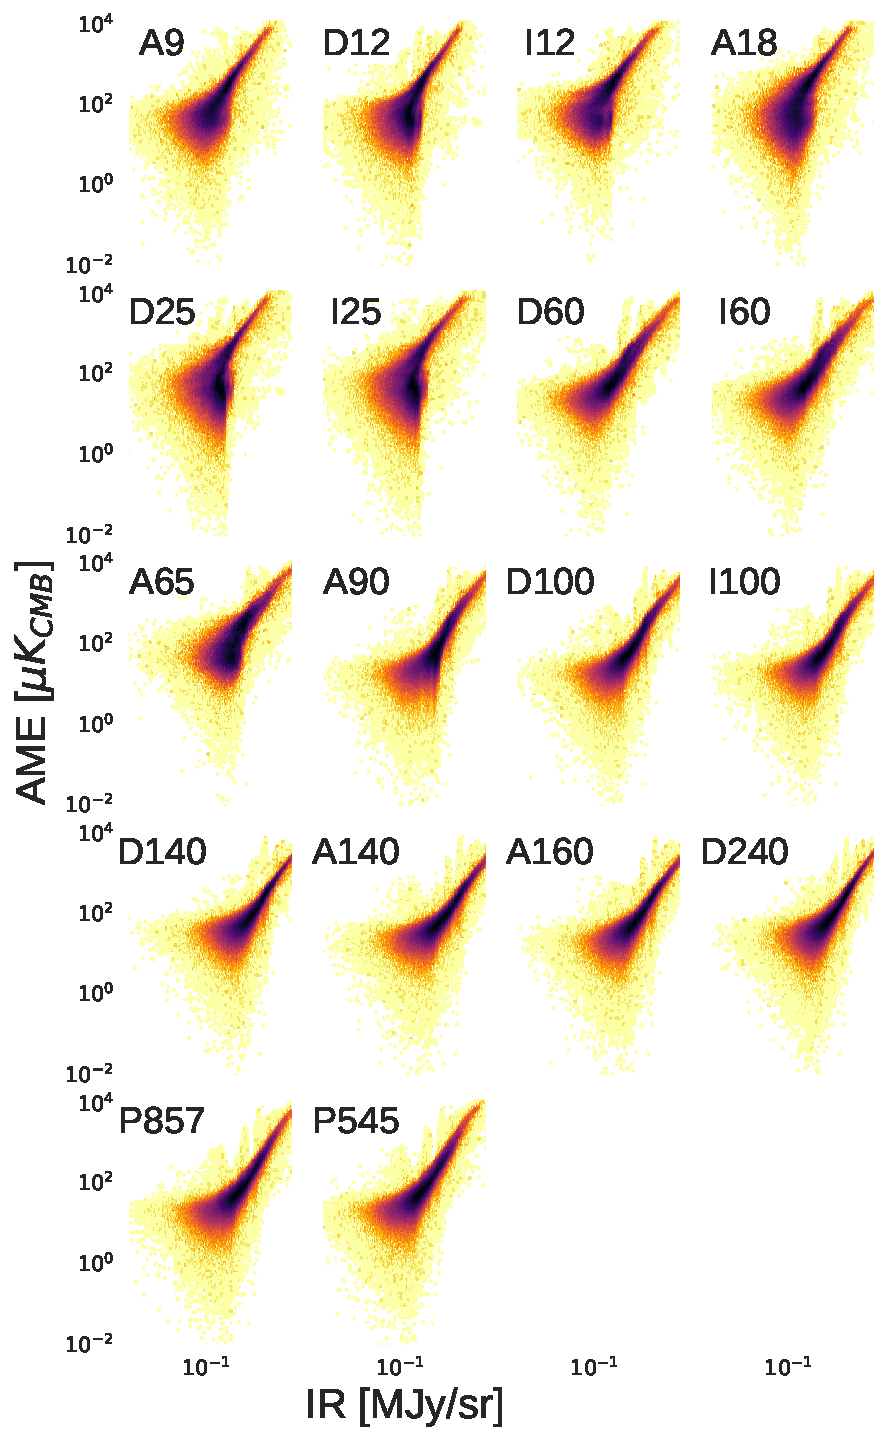
\includegraphics[width=150mm]{../Plots/AMEvsDust_allsky_allbands.pdf}
        \centering
        \caption{ALL-SKY kernel density estimates of 12-band infrared photometry against the PR2 AME map. Pixels within 10$^{\circ}$ of the ecliptic plane are excluded. 'A' indicates AKARI; 'D', DIRBE; 'I', IRAS, and 'P' Planck. The number after each letter indicates the band central nominal wavelength in microns (or frequency in GHz, in the case of the Planck bands.) }
      \end{figure*}

      \begin{figure*}
        \label{fig:AMEtoRvsDusttoR_allsky_allbands}
        \includegraphics[width=150mm]{../Plots/AMEvsDust_allsky_allbands__mpsub_Rnorm_kde.pdf}
        \centering
        \caption{Similar comparison to Fig. \ref{fig:AMEvsDust_allsky_allbands}, with both the IR and the AME intensities scaled by the PR2 dust radiance ($R$) for each pixel. }
      \end{figure*}

      \begin{figure*}
        \label{fig:Spearman_Map_nside8_AMEto}
        \includegraphics[width=80mm]{../Plots/Allsky_Corr/Spearman_Map_nside8_AMEtoA9.pdf}
        \includegraphics[width=80mm]{../Plots/Allsky_Corr/Spearman_Map_nside8_AMEtoI12.pdf}
        \includegraphics[width=80mm]{../Plots/Allsky_Corr/Spearman_Map_nside8_AMEtoI25.pdf}
        \includegraphics[width=80mm]{../Plots/Allsky_Corr/Spearman_Map_nside8_AMEtoA140.pdf}
        \includegraphics[width=80mm]{../Plots/Allsky_Corr/RadNorm/Spearman_Map_nside8_AMEtoA9.pdf}
        \includegraphics[width=80mm]{../Plots/Allsky_Corr/RadNorm/Spearman_Map_nside8_AMEtoI12.pdf}
        \includegraphics[width=80mm]{../Plots/Allsky_Corr/RadNorm/Spearman_Map_nside8_AMEtoI25.pdf}
        \includegraphics[width=80mm]{../Plots/Allsky_Corr/RadNorm/Spearman_Map_nside8_AMEtoA140.pdf}
        \centering
        \caption{Spatial map of Spearman correlation coefficients between the AME and IR intensity for 4 bands:$9~\mu{}m$, $12~\mu{}m$, $25~\mu{}m$, and $140~\mu{}m$. $S$ is calculated for all NSIDE 256 pixels within each NSIDE 8 pixel-sized bin.}
      \end{figure*}

\chapter{Analysis of the $\lambda$~Orionis Region}


% some references to get things started:
%http://www.sea-astronomia.es/drupal/sites/default/files/archivos/tesis/Bayo_tesis.pdf
%that one from wikipedia using WISE data


	Having looked at AME vs. dust emission on a course scale, we now introduce our analysis of a particular region. The $\lambda$~Orionis molecular ring \footnote{Also known as the Meissa Ring}, \citep{maddalena86,maddalena87}, is a particular AME-dominated region with a resolvable topology even at ~1$^{\circ}$ angular resolution. The region is shown in Figure \ref{fig:orionis-akari9} as it appears in 1$^{\circ}$ smoothed AKARI 9~$\mu$m data\footnote{Images at each wavelength used here are included as in appendix to this thesis}. The ring structure itself indicates excess microwave emission attributed to AME, however the central region is well-known to be dominated by free-free emission \citep{bayo12, koenig15,planck15XXV}. At approx. 10$^{\circ}$ wide, we can see the outline of the structure even in the low (1$^{\circ}$ FWHM) resolution Planck-COMMANDER AME map. At this resolution,This is one of the only coherent structures on the sky with a well-resolved shape; the molecular cloud ring, perhaps originating from a supernova remnant is distinguishable from the ionized region at its center. . In order to shift towards an investigation of individual AME-prominent regions, we have carried out an initial comparison of the AME of this region with its mid to far-IR dust emission.

	Figure \ref{fig:orionis-img} shows the region in 12 photometric bands, from the mid to far IR. Contours indicate the region's shape in the Planck PR2 AME map. Figure \ref{fig:orionis-corr} shows IR to AME cross correlation plots, for all pixels within the 10$^{\circ}$ by 10$^{\circ}$ $\lambda$~Orionis region. The correlation is most clear for the shortest and for the longest wavelength bands, and weakens the most at around 60~$\mu$m. The weakening of the correlation score appears to come from brighter 25 to 90~$\mu$m emission within the ring, while the ring structure itself appears relatively consistent accross all bands.

\begin{figure*}
  \label{fig:orionis-akari9}
  \includegraphics[width=150mm]{../Plots/LOri_akari9_AMEcont_1dres.pdf}
  \centering
  \caption{$\lambda$~Orionis as it appears in the AKARI 9~$\mu$m data. Contours indicate the AME, as given by the Planck PR2 AME map. The image is smoothed to a 1$^{\circ}$ PSF (much larger than the original 10 arcsec map. The $\lambda$~Orionis star itself is approximately located at the center of the image.
  %The dust wave structure, described by *citation needed*, is apparent, and seems to coincide with a local maxima in the PR2 AME contours. The units are MJy/sr. )
  }
\end{figure*}

\begin{figure*}
  \label{fig:orionis-img}
  \includegraphics[width=170mm]{../Plots/lOrionis_grid_img.png}
  \centering
  \caption{A grid of thumbnails showing the $\lambda$~Orionis region's structure, at 12 wavelengths, along with AME contours (shown in white countours. Spatial correlation seems to be the best at the shortest and longest wavelengths (AKARI/IRC 9~$\mu$m and Planck/HFI 550~$\mu$m). The images are smoothed and interpolated for demonstration. Figure \ref{fig:orionis-akari9} demonstrates the actual pixel grid used for the SED fitting and intensity correlation tests.}
\end{figure*}

\begin{figure*}
  \label{fig:orionis-corr}
  \includegraphics[width=170mm]{../Plots/orionis_correlations_AME.png}
  \centering
  \caption{Pixel cross-correlation for all pixels in the $\lambda$~Orionis cut-out region.  $S$ indicates the Spearman rank correlation coefficient for each plot.}
\end{figure*}

\subsubsection{SED Fitting}

We performed a full dust SED fitting on the LOri photometry, according to the \cite{galliano11} dust model. We used a mixture of amorphous carbon and silicate dust. Indeed, this dust mixture is more emissive than the standard silicate-graphite \citep{draine07}, by a factor of 2-3. As was shown by Herschel, in the LMC \citep{galliano11}, and by Planck, in the Milky Way \citep{planck16}, this increase of emissivity is necessary to have a proper fit of the sub-mm emission. We assume that the radiation field heating this dust mixture is the Galactic ISRF \citep{math83}, scaled by a factor $U$. We also assume, following \cite{dale01}, that the dust is exposed to a distribution of starlight intensity, distributed as:

\begin{equation}
   \label{eq:U}
     dM_{dust}\propto{} U^{-\alpha}dU
\end{equation}

between $U_{min}$ and $U_{max}$, where $U_{min}$, $U_{max}$ and $\alpha{}$ are free parameters. An old stellar population template (PEGASE; \citep{fioc97}) is added to this SED in order to model the near-IR emission. We perform a simple least-squares analysis. For the vast majority of the samples, the fits are reasonable, with the $\chi{}^{2}$ distribution shown in Fig. \ref{fig:AME_PCXVvsPR2}.

\chapter{Discussion}
  \label{ch:discussion}

  We have compared AME with infrared dust emission from 2 approaches. The results and discussion contained here apply to an angular scale of approximately 1$^{\circ}$. In general, our results support an AME-from-dust hypothesis. At 1$^{\circ}$ angular resolution, we do not find evidence that the AME is exclusively carried by PAHs. The correlation of far IR dust emission with AME appears to be the best predictor, with MIR/PAH emission being marginally more weakly correlated with AME. As far as the MIR bands are concerned, at least in terms of intensity, $I_{9\mu{}m}$ shows the strongest correlation. This result is mirrored in LOri, however in that case $I_{9\mu{}m}$ and $I_{545 \mu{}m}$ show the strongest correlation. In the case of $\lambda$~Orionis, AME vs. PAH emission is at least as strong as AME vs. FIR emission.

      \subsection{AME:Dust}

        As noted in Section 1, previous studies found that the AME generally correlates at dust-related IR wavelengths \citep{ysard10b,planckXV, hensley16}. We see the same overall pattern in the present study, for both the all-sky pixel-based analysis, and the inspection of the $\lambda$~Orionis region.

         In our all-sky comparison, we find a first-order correlation between IR intensity and AME intensity, for each of the 12 wavelengths sampled. This is again consistent with the previous investigations of the AME cited above, in that the FIR emission shows the tightest correlation with the AME intensity.

         In testing for a second-order correlation, we divided the IR intensities and AME intensity by the dust radiance, and again performed the band-by-band all-sky comparison. There is evidence of a residual correlation between $I_{MIR}$ and $I_{AME}/R$. Unsurprisingly, the strong correlation between $I_{FIR}$ and $I_{AME}$ disappears when scaling by $R$, as the the FIR bands are dominated by thermal dust emission. In this case, we again find no evidence of an improved correlation for the PAH-dominated bands.

        %In the case of the AME candidate regions, do we find evidence of a statistically stronger relationship between AME and total dust mass than AME vs. PAH mass, for the full set of 98 regions. We were able to confirm that the correlation coefficients are statistically distinct, via boostrap re-sampling (with replacement.) However the difference is marginal. Moreover the full set of 98 regions includes many regions that are either near the galactic plane, or do not have a strong S/N for the AME component separation. A similar result is found when we compare AME to the total dust luminosity and PAH luminosity.

        The closeness of the correlation coefficients found here is consistent with the results of the IRAS vs. AME correlation test result from \cite{planckXV}. They found that the correlation coefficient among the 4 IRAS bands (12, 25, 60, and 100~$\mu$m) differ from one another only by about 5\%, across the whole set of 98 regions. The trend of AKARI MIR and FIR data vs. the AME does not disagree with their IRAS comparison. This work adds that bands longer than IRAS 100~$\mu$m also correlate strongly with AME, especially the two Planck/HFI bands used.

      \subsection{AME:PAH}

        In the case of $\lambda$~Orionis we found that accross the whole region, AKARI 9~$\mu$m emission and Planck 545~GHz emission were the most strongly correlated with AME, having Spearman coefficients of 0.81 and 0.80. The results may be consistent with a scenario in which PAH mass, cold dust, and the AME are all tightly correlated. Weaker correlation from 25 to 70~$\mu$m may indicate that AME is weaker in regions of warmer dust and stronger radiation fields. This would be consistent with PCXV wherein highly significant AME regions tended to have a lower dust temperature than other regions. The fact that the correlation strengths of PAH-tracing mission the FIR emission are similar is in-line with what we have seen in \cite{ysard10b} and \cite{hensley16}. In those works, the two relationships (MIR vs. AME and FIR vs. AME) are very close, although these two papers are odds as to which relationship is stronger, and thus in their final interpretation. However in the investigation of the Perseus molecular cloud complex by \cite{tibbs11}, PAH emission (as well as VSG emission and hydrogen column density, $N_{H}$) does not show a strong correlation with AME compared to environmental paramters, such as dust temperature.

        On an all-sky basis, each of the bands sampled show correlation with the AME, however the FIR bands always show the strongest correlation. In fact, the correlation pattern of AME vs. each of the IR bands, very strongly resembles the correlation results of the Planck HFI bands vs. all of the other bands (Fig. \ref{fig:AME_IR_crosscorr_allbandsg}.) This is readily apparent from the pixel-density plots in Fig. \ref{fig:AMEvsDust_allsky_allbands}, wherein the FIR bands pixels show a very similar density profile vs. the AME. In attempting to factor out this first-order correlation, dividing the AME and IR intensities by the dust radiance for each pixel, we find the there is still a residual correlation between the MIR bands and the AME. The FIR bands scaled by the dust radiance, as expected, lack correlation with $I_{AME}/R$.


      \subsection{AME:$T$, $G_{0}$}

        According to spinning dust theory outlined in \cite{draine98a} and in subsequent works by \cite{ysard10a}, the AME profile and intensity will depend in part on the ISRF- but as is well-stated in \cite{hensley17a}, exactly how the ISRF will affect the AME SED is a more complicated question. Absorbed starlight photons may be able to rotationally excite the carriers, but if an enhanced ISRF leads to increased dust heating, then the increased IR emission can rotationally de-excite the carriers. However the ISRF affects not only the dust temperature but ionization of the carriers.

        \cite{hensley16} looked at the $AME$/$R$ ratio vs. $T$ and found only a slight anti-correlation of $P = -0.06$.

      \subsection{Microwave foreground component separation}

        There are known degeneracies between the foreground parameters of the COMMANDER maps (spinning-dust, and free-free, synchrotron components as described in \cite{planck15X}.) This can be demonstrated by comparing the ratio map of the PCXV intensity to thermal dust intensity.

\chapter{Summary}

  From these results, we cannot confirm or rule out a spinning-PAH hypothesis on an all-sky, 1$^{\circ}$ scale. While nanosilicates or magentic dipole emission from dust may be plausible contributors to the AME, as shown in \cite{hoang16a, hensley17a}, we do not find (at least at resolutions considered here) that PAHs can be ruled-out as a carrier. While it is true that the FIR in our study has a tighter correlation with AME than PAH-related bands, the correlation with PAH emission remains. This is true both when considering AME intensity to Either this is a coincidental correlation- PAHs and AME are both correlated with the ``actual'' carrier/s of AME, MIR phometric bands are not as good of a tracer of the actual PAH mass as we believed, or perhaps that PAHs are indeed contributing to the AME but that they are just one of multiple sources of the AME.

   If it can be shown that IR emission from non-PAH small dust particles, such as nanosilicates strongly correlates with the AME, another very interesting question would need to be addressed: why does PAH emission \textit{not} show a strong correlation? Do PAHs not have the range of dipole moments needed to produce emission in the 10 - 90 GHz range? Because, as is described in \cite{draine98a} and again in \cite{hensley17b}, such small particles should be spinning at the frequencies consistent with AME. Thus if we believe a particular class of small dust particles to exist, PAHs, nanosilicates, or otherwise- then they must be producing microwave emission, unless they do not have a permanent electric dipole.

  If there is a sufficient abundance of PAHs with an electric dipole, then we must consider the possibility that the data currently available to do not offer the necessary spatial resolution, or that the photometric bands used do not allow us to adequately separate the individual dust components (i.e. the PAH features from potential nanosilicate features) and/or microwave foreground emission components (free-free from spinning-dust.) We look forward to continued environment-resolved comparisons to investigate the potential AME-PAH (or AME-nanosilicates, iron nanoparticles) relationship in a region by region, especially given the disagreement we find between our examination of lambda Orionis and the all-sky analysis.


 This project is supported by JSPS and CNRS under the Japan--France Research Cooperative Program. We would like to give special thanks to the AME Workshop 2016 attendees and organizer, Chris Tibbs, for enlightening disucssions. Thanks also to Nathalie Ysard and Steven Gibson, and the staff of Grid, Inc. for helpful feedback.

\chapter*{Acknowledgements}
\addcontentsline{toc}{chapter}{Acknowledgements}
     I would like to thank Professor Takashi Onaka firstly for guiding me since I first came to his laboratory as an undergraduate summer intern, in June 2012. I'm not sure if I've worked hard enough for the honor of being his last Ph.D. student, but its been a pleasure. I am extremely happy that I to complete my degree here. I wish him the happies of retirements, while sincerely doubting he will be able to stay away from research for long.

     Onaka-sensei and the members of the Onaka-lab have literally helped me to survive here, assisting any time that I have had difficulty adjusting as a foreign student.

    Itsuki Sakon has helped me greatly from the moment I arrived in Japan (literally.) It is also quite refreshing when his driving skills leave me at my destination much earlier than planned.

     I have been very lucky to have helpful co-authors for the various posters and abstracts I have presented in the course of this thesis: Ho-Gyu Lee, Daisuke Ishihara, Yasuo Doi, Ho-Gyu Lee, Mark Hammonds, Fumihiko Usui, Takafumi Ootsubo, Ryou Ohsawa, Tamami Okada, Hidehiro Kaneda --- especially, my international collaborators kind enough to host me over the years, Ronin Wu, Mridusmita Buragohain, Rupjyoti Gogoi, Frederic Galliano, Amit Pathak, Martin Giard, and Olivier Berne.

     My undergraduate advisor, Steven Gibson, deserves a special thanks for continued kind encouragement and research advice even now that I have graduated from WKU.

     Most personally, I must thank my mother, Catherine Marie Bell who has supported me more than seems possible for a single human being. The same goes to my younger siblings, Joseph, Emma, Caleb, and Noah who I have too few opportunities to help grow up. I thank also Deborah and Faithie (``Mama'') Guffy, who have been like aunt and gradnmother to us all.

     My day to day life in Japan has been brightened by partner of five years, Yuki Sugisawa \begin{CJK}{UTF8}{min}(杉澤友紀)\end{CJK}. His family too, who have been an unofficial host-family over the years, Chikako \begin{CJK}{UTF8}{min}(千賀子様),Hiromi (宏美様), Takeshi (剛様), and Chiri\end{CJK}. Even his grandmother Junko and grandfather Sadao Masuda \begin{CJK}{UTF8}{min}(桝田順子と定雄様)\end{CJK} have shown me much kindness during my visits to Osaka.

     A special note of thanks is owed to my friends who have inspired me and shared moral support, from back in the US, throughout my program: Alexandria Boswell, Hannah Kagan-Moore, Alexander Chen, George Johnson, Nicolas Tarantino, and John Max Wilson; as well as my classmates at U.Tokyo, Scarlet Elgueta, Jerome de Leon, Ryouta Kawamata, Takahiro Sudoh, Taku Okamura, John Livingston, Kyle Mede, Yuta Kato, and others.

     This project could not have found its way to any assemblance of completion without kind and insightful discussions with Nathalie Ysard, Alessandra Candian,  Chikako Yasui, Norita Kawanaka, Bruce Draine, Chris Tibbs, Francois Boulanger, Brandon Hensley, Clive Dickinson, Yasushi Suto, Othman Benomar, and Anthony Jones.

     The staff of GRID, Inc., especially Mehdi Shibahara and Ying-Ming Chen, helped guide my career choices and advance my knowledge of machine learning besides being the best lunch pals.

     I wish the best of luck to my kohais in Onaka-lab: Izumi Endo, Jin Zhang, Tomoyuki Kimura, Ayato Ikeuchi, and Mingie Jian in their continued studies and careers. I also want to express special thanks to the staff of the International Liaison Office, for advising me over the last five years, even since I was an undergraduate research internship student, in the UTRIP program of 2012.

     This project acknowledges a wide range of authors. I would like also to credit especially any of those whose names did not make it into the literature, for whatever reason. Especially the many women and minorities who have made direct or indirect contribtuions to science, but have been systematically overlooked and underrepresented in journals and awards.

     My financial support for living and tuition expenses during this time has been generously provided by "MEXT", the Ministry of Education, Culture, Sports, Science and Technology (\begin{CJK}{UTF8}{min}文部科学省.\end{CJK}). This research is based on observations with AKARI, a JAXA project with the participation of ESA; Planck (http://www.esa.int/Planck), an ESA science mission with instruments and contributions directly funded by ESA Member States, NASA, and Canada; and IRAS, a joint project of the US, UK and the Netherlands.

    This research made use of Montage. It is funded by the National Science Foundation under Grant Number ACI-1440620, and was previously funded by the National Aeronautics and Space Administration's Earth Science Technology Office, Computation Technologies Project, under Cooperative Agreement Number NCC5-626 between NASA and the California Institute of Technology


\small
\bibliographystyle{apj}
\bibliography{reference}
\end{document}
